\documentclass[conference]{IEEEtran}
\IEEEoverridecommandlockouts
% The preceding line is only needed to identify funding in the first footnote. If that is unneeded, please comment it out.
\usepackage{cite}
\usepackage{amsmath,amssymb,amsfonts}
\usepackage{algorithmic}
\usepackage{graphicx}
\usepackage{textcomp}
\usepackage{xcolor}
\usepackage{hyperref}
\def\BibTeX{{\rm B\kern-.05em{\sc i\kern-.025em b}\kern-.08em
    T\kern-.1667em\lower.7ex\hbox{E}\kern-.125emX}}
%\usepackage{biblatex}
    
%encoding
%--------------------------------------
\usepackage[T1]{fontenc}
\usepackage[utf8]{inputenc}
%--------------------------------------

%Portuguese-specific commands
%--------------------------------------
\usepackage[portuguese]{babel}
%--------------------------------------

%Hyphenation rules
%--------------------------------------
\usepackage{hyphenat}
\hyphenation{mate-mática recu-perar}
%--------------------------------------  
    
\begin{document}

\title{Aprendizagem Automática e COVID-19\\
}

\author{\IEEEauthorblockN{Bruno Carvalho}
\IEEEauthorblockA{\textit{Departamento de Engenharia Informática} \\
\textit{Instituto Superior de Engenharia do Porto}\\
Porto, Portugal \\
1200145@isep.ipp.pt}
\and
\IEEEauthorblockN{Sofia Canelas}
\IEEEauthorblockA{\textit{Departamento de Engenharia Informática} \\
\textit{Instituto Superior de Engenharia do Porto}\\
Porto, Portugal \\
1200185@isep.ipp.pt}
}

\maketitle

\begin{abstract}
Através de dados retirados de uma base de dados internacional, pretende-se prever o impacto da pandemia na população mundial seguindo processos de aprendizagem automática e posterior avaliação dos mesmos.
\end{abstract}

\begin{IEEEkeywords}
análise, dados, COVID-19, pandemia, exploração, inferência, correlação, regressão, classificação, aprendizagem automática, árvores de decisão, redes neuronais, knn, avaliação
\end{IEEEkeywords}

\section{Introdução} %-------------------------------------
No âmbito da pandemia atual, foram extraídos da base de dados internacional “Our World in Data” \cite{database}, dinamizada pela Johns Hopkins University (JHU), dados reais incidentes em 206 países, contendo indicadores acerca da população dos mesmos. 
Pretende-se, recorrendo a processos de aprendizagem automática, prever o impacto da COVID-19 na população mundial, com o objetivo de avaliar os algoritmos quanto à sua aproximação à realidade. Para isso, serão utilizados modelos de regressão e classificação, nomeadamente regressão linear simples e múltipla, árvores de regressão/decisão, redes neuronais e k-vizinhos-mais-próximos (KNN).



\section{Metodologia de Trabalho}
\label{methodology} %-------------------------------------
Tendo por base o ficheiro “countryaggregatedata.csv”\cite{dataFile}, foi criado um script em R separado em dois tipos de modelos: Regressão e Classificação. Em cada um destes estão presentes alíneas independentes que utilizam algoritmos de aprendizagem automática sobre os dados referentes ao ficheiro. Após a conclusão das diferentes alíneas, foi realizada a comparação e avaliação dos algoritmos, onde a discussão de resultados se encontra nas secções \ref{regression} e \ref{classification} deste artigo. 



\section{Revisão do Estado da Arte} %-------------------------------------
A aprendizagem automática divide-se em três áreas, sendo estas a \textit{Supervised Learning}, \textit{Unsupervised Learning} e \textit{Reinforcement/Semi-Supervised Learning} \cite{algorithms}.
Na área de \textit{Supervised Learning} os modelos são construídos tendo em conta um processo de treino onde o algoritmo calcula as previsões e recebe o resultado correto, comparando-o, posteriormente, com a previsão obtida. Alguns destes algoritmos são os de regressão e classificação: Regressão Linear, Modelo KNN, Árvores de Decisão, Redes Neuronais, entre outros \cite{regressionalgorithms}.
Relativamente à \textit{Unsupervised Learning}, os modelos tentam criar estruturas através dos dados de \textit{input}, com o objetivo de organizar os dados por semelhança. Alguns dos algoritmos presentes nesta área são do tipo de \textit{Clustering} \cite{clusteringalgorithms} e de Aprendizagem por Regra de Associação \cite{associationrulealgorithms}.
A última área referida reúne os objetivos das áreas referidas anteriormente, ou seja, procura organizar os dados em estruturas por semelhança e também fazer previsões dos mesmos. Os algoritmos utilizados nesta área são extensões dos algoritmos de regressão e classificação, referidos anteriormente.
Para a avaliação dos algoritmos de aprendizagem automática destacam-se: a Matriz de Confusão, que sumariza a performance através dos termos “True Positive”, “True Negative”, “False Positive” e “False Negative”; os valores da \textit{Accuracy}, \textit{Precision}, \textit{Recall} e \textit{F1 score}, que são calculados através da matriz de confusão, \textit{Threshold}; \textit{AUC-ROC}; entre outros. Os algoritmos de regressão contêm medidas próprias para a sua avaliação sendo estas o Erro Absoluto Médio (MAE), Erro Quadrático Médio (MSE), Raiz do Erro Quadrático Médio (RMSE) e o R quadrado \cite{evaluationmetrics}.



\section{Exploração e Preparação dos Dados} %-------------------------------------
No início do script em R estão presentes as importações de bibliotecas necessárias para a realização dos algoritmos, avaliações e testes utilizados. De seguida, encontram-se funções criadas para calcular valores de avaliação dos algoritmos, assim como para visualização dos mesmos na consola.
Como já referido na secção \ref{methodology}, o script está organizado por duas partes (Regressão e Classificação), cada uma contendo alíneas em que são utilizados algoritmos diferentes e feitas comparações e/ou avaliações. Nestas alíneas são obtidos os dados de treino e teste e a sua posterior incorporação nos algoritmos. Na parte final é feita a avaliação do algoritmo utilizado e, no caso de ser mais do que um, é feita a comparação entre os mesmos.
De forma a igualar a dimensão dos dados de treino e teste perante todos os algoritmos, utilizou-se o critério \textit{holdout} 70\% treino e 30\% teste em todos os pontos, onde também foram eliminadas as colunas “continent” e “location” uma vez que o algoritmo de redes neuronais não é capaz de processar dados classificados (em texto) e, também, devido à falta de relevância que estes possuem sobre os algoritmos utilizados. Assim, todos os algoritmos utilizam os mesmos dados de teste em cada ponto para uma comparação justa.




\section{Análise e Discussão de Resultados: Regressão}
\label{regression} %-------------------------------------

\subsection{Carregamento do ficheiro, dimensão e sumário dos dados.} 
\label{ex01}
Após a importação dos dados contidos no ficheiro, é possível verificar a sua dimensão, sendo esta de 209 linhas (cada uma referente a um país) e 25 colunas, referentes a indicadores acerca da população.
\begin{figure}[htbp]
\centerline{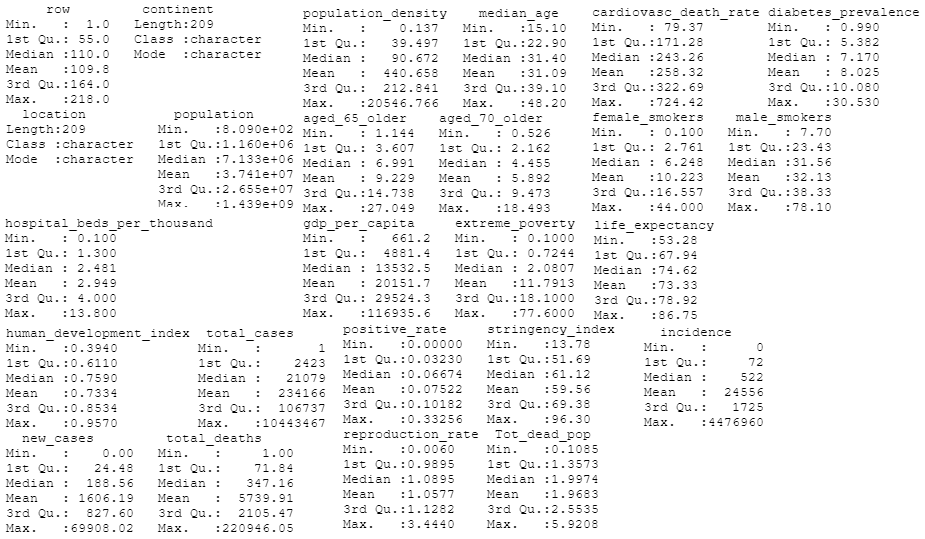
\includegraphics[width=0.95\columnwidth]{images/01.png}}
\caption{Sumário dos dados importados}
\label{summary}
\end{figure}
\begin{equation}
y = \frac{y-min_{y}}{max_{y}-min_{y}} \label{norm}
\end{equation}
Através do sumário dos dados (Fig. \ref{summary}) é possível perceber que estes precisarão de ser normalizados para serem incluídos nos algoritmos de redes neuronais e knn, pelo que se procedeu à normalização dos mesmos através da função representada pela equação \eqref{norm}.
Na normalização dos dados foram excluídas as colunas “continent” e “location” por não apresentarem relevância na aprendizagem automática e por não serem dados numéricos. Estes dados foram utilizados ao longo dos pontos do artigo onde a sua inclusão no algoritmo era necessária.


\subsection{Diagrama de correlação entre todos os atributos}
\begin{figure}[htbp]
\centerline{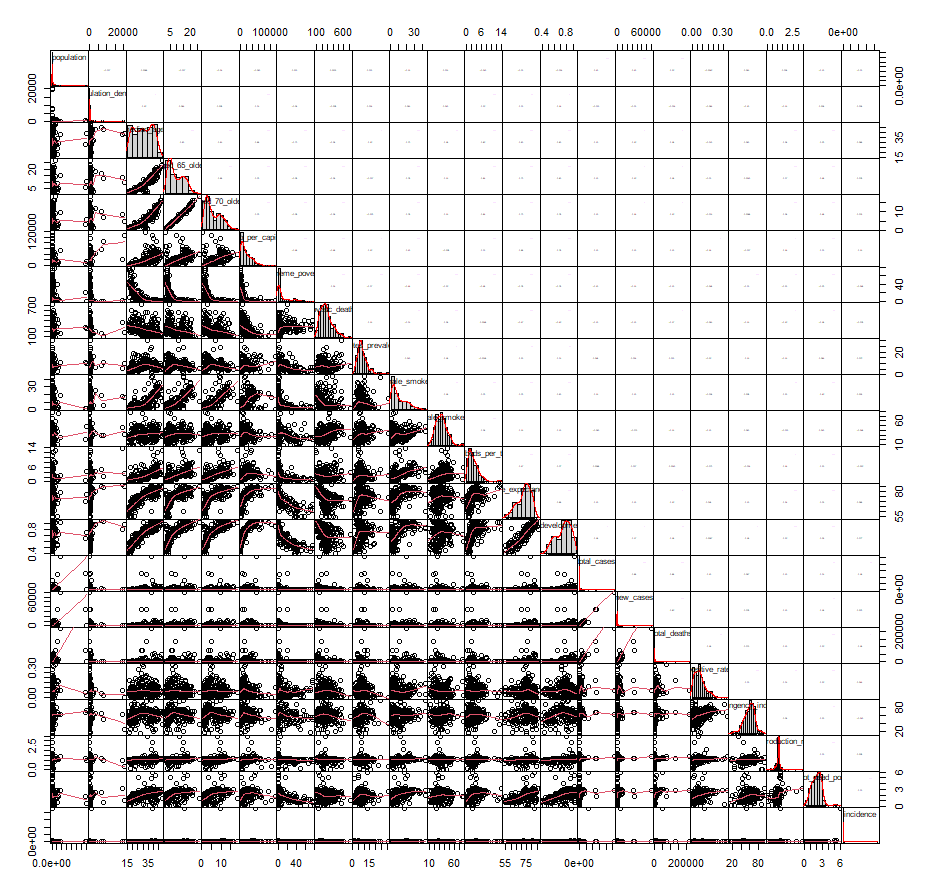
\includegraphics[width=0.95\columnwidth]{images/02_1.png}}
\caption{Matriz de correlação}
\label{02_1}
\end{figure}
Para a realização do diagrama de correlação entre todos os atributos procedeu-se à construção da matriz de correlação, presente na Fig.\ref{02_1}.

\begin{figure}[htbp]
\centerline{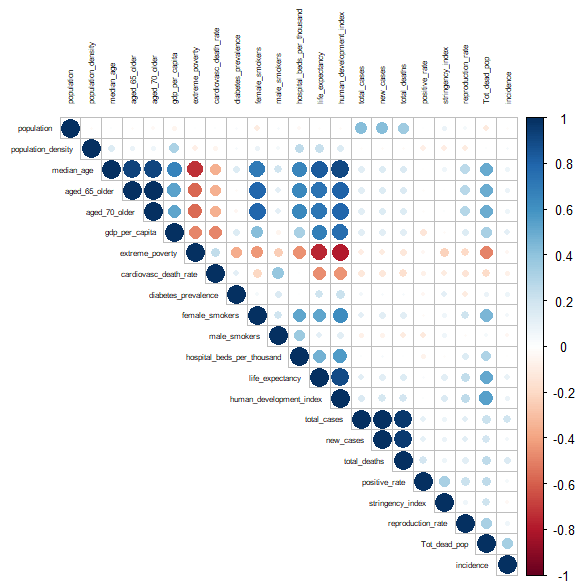
\includegraphics[width=0.95\columnwidth]{images/02_2.png}}
\caption{Visualização da matriz de correlação  através do correlograma}
\label{02_2}
\end{figure}
Para facilitar a visualização dos dados utilizou-se um correlograma que permite visualizar a matriz de correlação através de um sistema de cores e círculos, visível na Fig.\ref{02_2}, sendo que as cores azul e vermelho escuro pertencentes, respetivamente, aos valores 1 e -1, em conjunto com um círculo maior representam os melhores valores de correlação.
Analisando o correlograma, excluindo-se os atributos correlacionados consigo mesmos presentes na diagonal, verificam-se os seguintes pares de atributos com boa correlação:
\begin{itemize}
	\item "median$\_$age" e "aged$\_$65$\_$older"
	\item "median$\_$age" e "aged$\_$70$\_$older"
	\item "median$\_$age" e "extreme$\_$poverty"
	\item "median$\_$age" e "human$\_$development$\_$index"
	\item "aged$\_$65$\_$older" e "aged$\_$70$\_$older"
	\item "extreme$\_$poverty" e "life$\_$expectancy"
	\item "extreme$\_$poverty" e "human$\_$development$\_$index"
	\item "total$\_$cases" e "new$\_$cases"
	\item "total$\_$cases" e "total$\_$deaths"
	\item "new$\_$cases" e "total$\_$deaths"
\end{itemize}



\subsection{Regressão linear simples entre “new$\_$cases” e “total$\_$deaths”}

\subsubsection{Função linear resultante}
\begin{equation}
y = 1056.156 + 2.991x\label{3a_equation}
\end{equation}
\begin{equation}
R^{2}_{ajust.} = 0.6835\label{3a_r2ajust}
\end{equation}
\begin{equation}
p-value = 2.2*10^{-16}\label{3a_pvalue}
\end{equation}
Após a separação dos dados em dados de treino e teste, criou-se o modelo de regressão linear, cuja função obtida está apresentada em \eqref{3a_equation}. A interseção é 1056.156 e o declive 2.991. 
O R quadrado ajustado \eqref{3a_r2ajust} indica que a correlação entre os atributos "new$\_$cases" e "total$\_$deaths" não é muito forte, uma vez que o valor ainda se encontra afastado do valor 1. Isto significa que o modelo de regressão não é, de igual forma, muito forte.
Por fim, o p-value \eqref{3a_pvalue}, sendo inferior a 0.05, permite concluir que a análise realizada sobre o R quadrado ajustado é estatisticamente significativa


\subsubsection{Diagrama de dispersão e reta correspondente ao modelo de regressão}
\begin{figure}[htbp]
\centerline{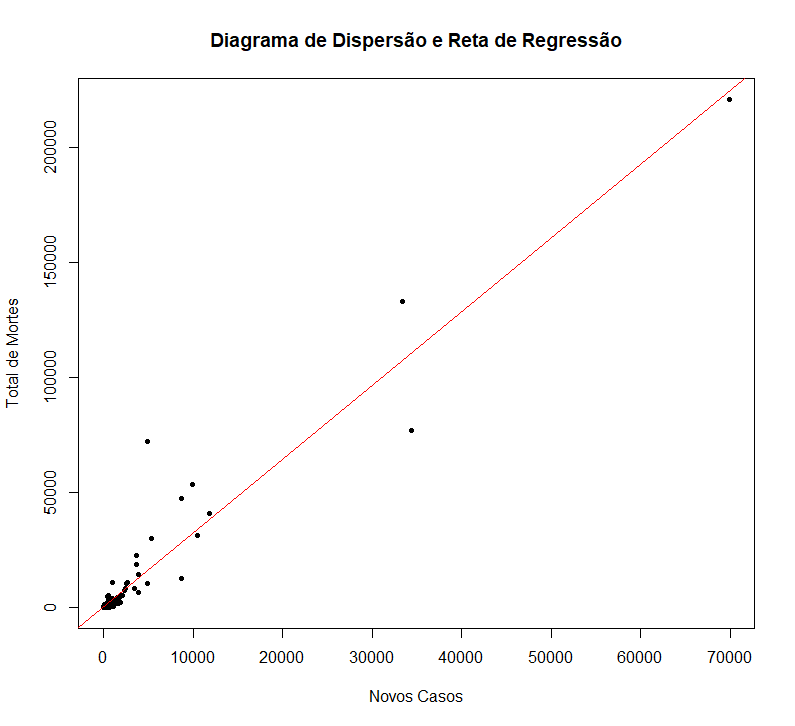
\includegraphics[width=0.95\columnwidth]{images/03.png}}
\caption{Gráfico de dispersão e reta de regressão linear}
\label{3a}
\end{figure}
Através do diagrama de dispersão da Fig. \ref{3a}, verifica-se que os pontos estão bastante dispersos em relação à reta correspondente ao modelo de regressão. Assim, não existe uma relação linear entre os dois atributos, tal como confirmado na alínea anterior.

\subsubsection{Erro médio absoluto (MAE) e raiz quadrada do erro médio (RMSE)}
\begin{equation}
MAE = 2051.678\label{3a_mae}
\end{equation}
\begin{equation}
RMSE = 4613.71\label{3a_rmse}
\end{equation}
Para finalizar, a avaliação do modelo de regressão linear é, efetivamente, negativa. Isto confirma-se não só pelo modelo não ser muito forte, como também pelos valores do MAE \eqref{3a_mae} e RMSE \eqref{3a_rmse} serem bastante altos.


\subsection{Previsão da esperança de vida aplicando regressão linear múltipla, árvore de regressão e rede neuronal.}
Utilizando os métodos de regressão linear múltipla, árvore de regressão e rede neuronal, pretendeu-se prever a esperança de vida através dos outros atributos presentes nos dados. Após a realização destes métodos, houve uma comparação entre todos com o objetivo de perceber aquele com melhor desempenho a prever a esperança de vida.

\subsubsection{Regressão linear múltipla}
Para a regressão linear múltipla utilizaram-se todos os atributos (excetuando o "continent" e "location", como referido anteriormente) para prever a esperança de vida.

\begin{figure}[htbp]
\centerline{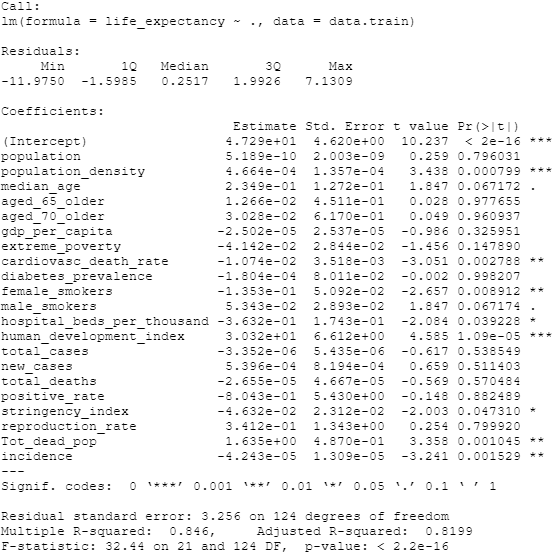
\includegraphics[width=0.95\columnwidth]{images/04_1.png}}
\caption{Resumo do modelo da função de regressão linear múltipla}
\label{4a}
\end{figure}

No sumário da função de regressão obtida, presente na Fig.\ref{4a}, observam-se os coeficientes obtidos e, também, que apenas os parâmetros da “population$\_$density”, “cardiovasc$\_$death$\_$rate”, “female$\_$smokers”, “hospital$\_$beds$\_$ per$\_$thousand”, “human$\_$development$\_$index”, “positive$\_$rate”, “Tot$\_$dead$\_$pop” e “incidence” é que têm relação linear com os valores da esperança de vida, uma vez que os seus p-values são inferiores a 0.05, logo, consideram-se estatisticamente significativos.

\begin{equation}
R^{2}_{ajust.} = 0.8199\label{4a_r2ajust}
\end{equation}
\begin{equation}
p-value = 2.2\times 10^{-16}\label{4a_pvalue}
\end{equation}

Os valores presentes nas equações \eqref{4a_r2ajust} e \eqref{4a_pvalue} permitem concluir, em primeiro lugar, que existe alguma correlação entre os atributos e a esperança de vida, dado que 0.8199 está algo próximo de 1 e, em segundo, que esta é estatisticamente significativa pois o p-value é inferior a 0.05.
Com a obtenção da função de regressão, testou-se a mesma com a previsão dos dados de teste, sendo que os valores do erro absoluto médio (MAE) e a sua raiz quadrada (RMSE) são os apresentados nas equações \eqref{4a_mae} e \eqref{4a_rmse}, respetivamente.

\begin{equation}
MAE=5.416697\label{4a_mae}
\end{equation}
\begin{equation}
RMSE=24.49499\label{4a_rmse}
\end{equation}


\subsubsection{Árvore de regressão}
A árvore de regressão para a variável da esperança de vida foi obtida com a função \textit{rpart} e com o método ANOVA. O resultado obtido é o apresentado na Fig.\ref{4b}.

\begin{figure}[htbp]
\centerline{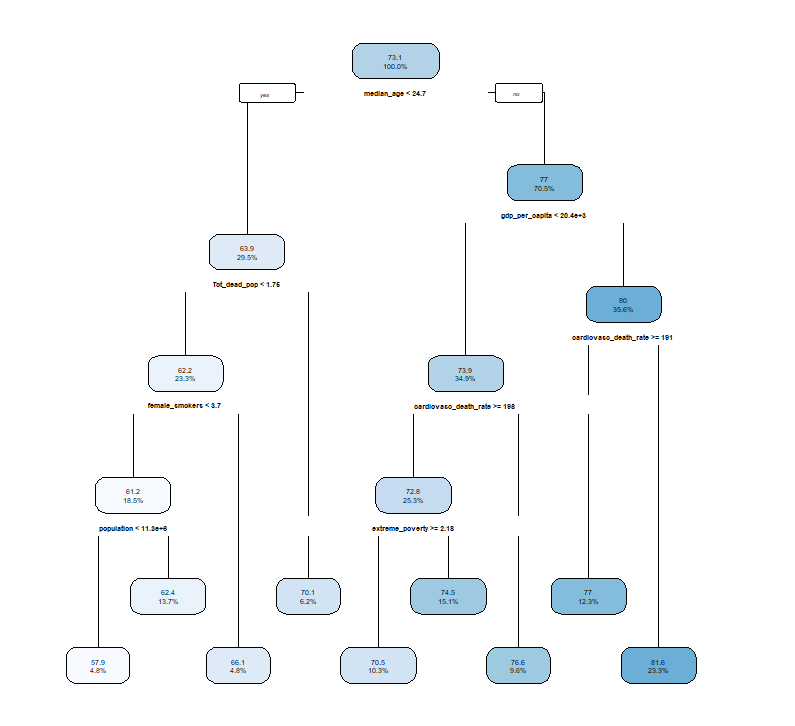
\includegraphics[width=0.95\columnwidth]{images/04_2.png}}
\caption{Árvore de regressão para a variável life$\_$expectancy}
\label{4b}
\end{figure}

Com a árvore de regressão construída, realizou-se a previsão e avaliação da mesma, sendo que foram obtidos os valores apresentados do erro médio absoluto (MAE) e a sua raíz quadrada (RMSE).

\begin{equation}
MAE=2.907016\label{4b_mae}
\end{equation}
\begin{equation}
RMSE=3.828154\label{4b_rmse}
\end{equation}


\subsubsection{Redes neuronais}
Através dos dados normalizados foram construídas três redes neuronais com parâmetros diferentes, sendo estes: uma rede com 1 nó interno; uma com 4 nós internos e uma com 2 níveis internos de 5 e 3 nós. Os resultados gráficos e matemáticos de cada rede são apresentados abaixo.

1 nó interno:
\begin{figure}[htbp]
\centerline{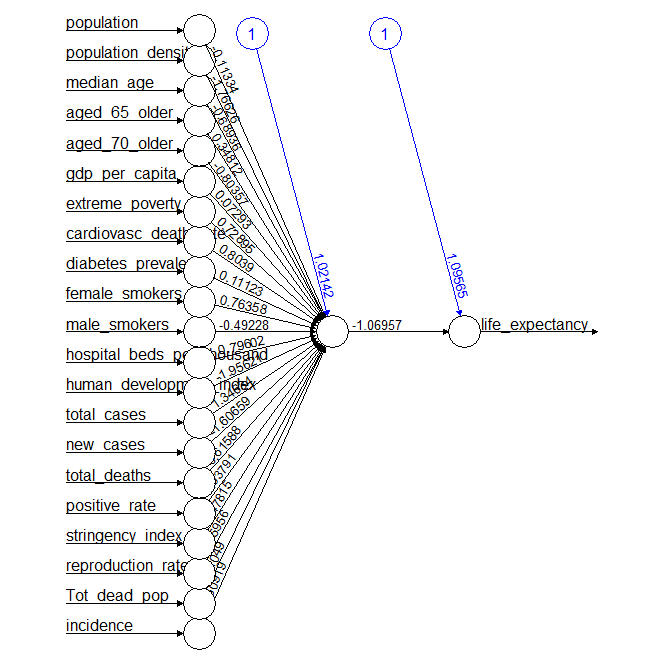
\includegraphics[width=0.95\columnwidth]{images/04_3.png}}
\caption{Rede neuronal com 1 nó interno para a variável life$\_$expectancy}
\label{4c1}
\end{figure}
\begin{equation}
MAE=0.08414757\label{4c1_mae}
\end{equation}
\begin{equation}
RMSE=0.1493318\label{4c1_rmse}
\end{equation}

4 nós internos:
\begin{figure}[htbp]
\centerline{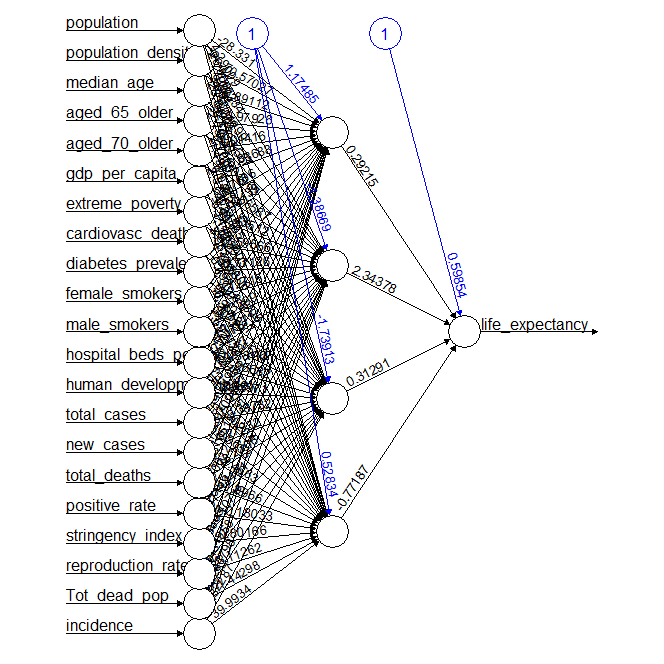
\includegraphics[width=0.95\columnwidth]{images/04_4.png}}
\caption{Rede neuronal com 4 nós internos para a variável life$\_$expectancy}
\label{4c2}
\end{figure}
\begin{equation}
MAE=0.09749222\label{4c2_mae}
\end{equation}
\begin{equation}
RMSE=0.1625733\label{4c2_rmse}
\end{equation}

2 níveis internos com 5 e 3 nós:
\begin{figure}[htbp]
\centerline{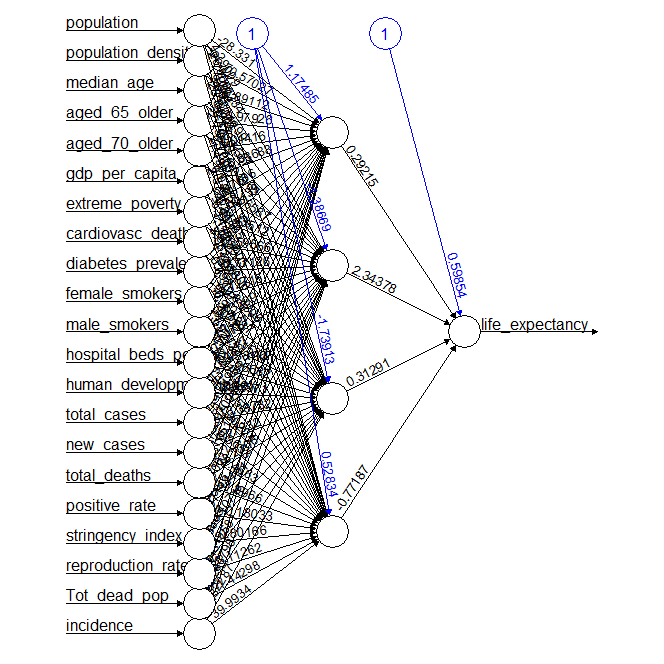
\includegraphics[width=0.95\columnwidth]{images/04_4.png}}
\caption{Rede neuronal com 5 e 3 nós internos para a variável life$\_$expectancy}
\label{4c3}
\end{figure}
\begin{equation}
MAE=0.09220327\label{4c3_mae}
\end{equation}
\begin{equation}
RMSE=0.2227114\label{4c3_rmse}
\end{equation}


Através dos erros calculados para cada rede neuronal é possível concluir que há uma perda na precisão da previsão com o aumento de níveis e nós internos, já que a melhor rede neuronal desta amostra é aquela com apenas um nó interno. Esta conclusão é retirada através dos RMSEs, onde a primeira rede apresenta um valor inferior às restantes.

Com os resultados obtidos nos três modelos realizados, é possível tirar conclusões referentes à eficiência de cada um deles. O modelo que apresenta um menor erro médio absoluto (MAE) é a rede neuronal com 1 nó interno, que resultou num erro médio muito inferior aos restantes modelos sendo, por isso, o melhor modelo destes três.
A regressão linear múltipla apresenta o pior erro médio, ou seja, a árvore de regressão foi o segundo melhor modelo ficando com um erro médio sensivelmente no meio dos valores do melhor e pior modelos.

\subsubsection{Teste aos resultados dos dois melhores modelos}
Por fim realizou-se um teste para comparar as médias dos erros dos dois melhores modelos, sendo estes a Árvore de Regressão e a melhor Rede Neuronal (1 nó interno).

\begin{equation}
Shapiro-Wilk_{p-value}=1.96\times 10^{-11}\label{4_shapiro}
\end{equation}
\begin{equation}
Lillierfors_{p-value}=6.656\times 10^{-13}\label{4_lillie}
\end{equation}
Antes de fazer o teste, verificou-se a normalidade dos dados através de um teste de Shapiro- Wilk e Lillierfors, que resultaram nos p-values apresentados em \eqref{4_shapiro} e \eqref{4_lillie}. Estes valores permitem concluir que os dados não têm distribuição normal pois ambos os valores são inferiores a 0.05.

\begin{equation}
p-value=1.221\times 10^{-5}\label{4_levene}
\end{equation}
Assim, há a implicação da realização de um t.test, já que os dados não apresentam normalidade. Com isto, realizou-se um \textit{Levene Test} para verificar as igualdades das variâncias, sendo que o resultado deste teste permite concluir que não o são, visto que o p-value é inferior a 0.05 \eqref{4_levene}.

\begin{equation}
  \begin{array}{l}
    H_{0}:\mu _{rpart} - \mu _{neural}=0 \\ 
    H_{1}:\mu _{rpart} - \mu _{neural}\neq 0
  \end{array}\label{4_hypothesis}
\end{equation}
\begin{equation}
p-value=1.214\times 10^{-5}\label{4_ttest}
\end{equation}
O teste foi realizado com as hipóteses referidas em \eqref{4_hypothesis} e tendo em conta a diferença das variâncias verificadas no \textit{Levene Test}. O resultado obtido permite concluir que há diferenças significativas entre as médias dos erros dos dois melhores modelos, a um nível de significância de 5\%, já que o p-value é inferior a 0.05.



\section{Análise e Discussão de Resultados: Classificação} 
\label{classification} % ------------------------------------------------------

\subsection{Derivação de um novo atributo NiveldeRisco, discretizando o atributo Taxa de Transmissibilidade, em 2 classes: low e high usando como valor de corte a média do atributo.}
\label{ex05}
Com o objetivo de separar os dados da Taxa de Transmissibilidade em duas classes, obteve-se o valor da média dos mesmos \eqref{5}.
\begin{equation}
\mu = 1.057654\label{5}
\end{equation}
Através deste valor foi possível fazer a separação dos dados, onde o valor de low ocorre em 75 países e o valor high ocorre em 134 países. Isto permite concluir que a maioria dos países presentes nos dados têm um índice de transmissibilidade superior a 1 e superior à própria média dos países.


\subsection{Avaliação da capacidade preditiva, através do k-fold cross validation, relativamente ao novo atributo NiveldeRisco usando árvore de regressão, rede neuronal e k-vizinhos-mais-próximos.}
\subsubsection{Árvore de decisão}
\begin{figure}[htbp]
\centerline{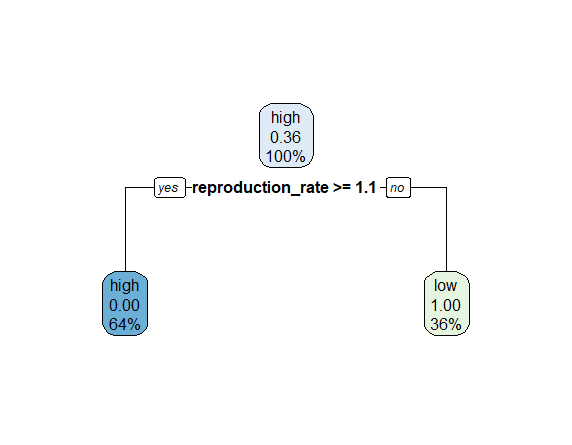
\includegraphics[width=0.95\columnwidth]{images/06_1.png}}
\caption{Árvore de decisão para a varíavel NiveldeRisco}
\label{6a_rpart}
\end{figure}
\begin{equation}
Accuracy = 0.984127\label{6a_accuracy}
\end{equation}
Com a criação do novo atributo NiveldeRisco, procedeu-se à criação de uma árvore de regressão que pretende prever o mesmo, estando o resultado da árvore o presente na Fig. \ref{6a_rpart} e a avaliação da mesma através da accuracy na equação \eqref{6a_rpart}.


\subsubsection{Rede neuronal}
\begin{figure}[htbp]
\centerline{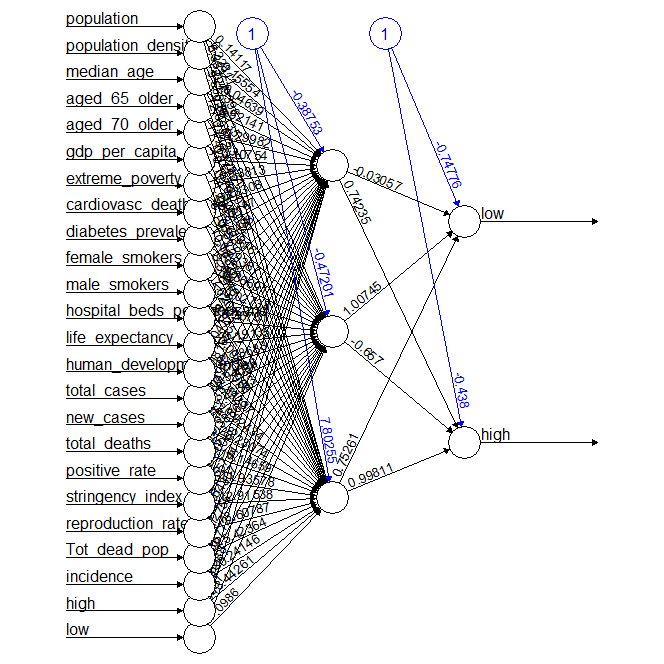
\includegraphics[width=0.95\columnwidth]{images/06_2.png}}
\caption{Rede neuronal com 3 nós internos para a varíavel NiveldeRisco}
\label{6b_neural}
\end{figure}
\begin{equation}
Accuracy = 1\label{6b_accuracy}
\end{equation}
Após a criação da árvore de regressão, construiu-se uma rede neuronal com 3 nós internos, presente na Fig. \ref{6b_neural}, e obteve-se o respetivo valor de accuracy \eqref{6b_accuracy} para posterior avaliação e comparação.


\subsubsection{K-vizinhos-mais-próximos}
\begin{equation}
k = round(\sqrt{nrow(dadosteste)})=12\label{6c_k}
\end{equation}
\begin{equation}
Accuracy = 1\label{6c_accuracy}
\end{equation}
Por último, utilizou-se o algoritmo knn com k igual ao demonstrado na equação \eqref{6c_k} \cite{knn} e calculou-se novamente a accuracy do modelo, sendo esta disposta na equação \eqref{6c_accuracy}.


\subsubsection{k-fold cross validation}
Os dois melhores algoritmos entre os três realizados são a rede neuronal e o knn, uma vez que possuem uma taxa de acerto perfeita, em comparação com a árvore de decisão que apresenta um valor bastante bom, mas não perfeito.
Com isto, procedeu-se a uma posterior avaliação usando o método k-fold cross validation para estes dois melhores modelos. Na rede neuronal, a taxa de acerto média obtida foi de 99.68\% e o seu desvio 0.004. Relativamente ao modelo knn, a taxa de acerto média foi de 87.07\% e desvio 0.168. Assim, a rede neuronal apresenta melhores resultados, mesmo em várias repetições, relativamente ao knn, sendo considerado o melhor algoritmo destes três.


\subsubsection{Teste aos resultados dos dois melhores modelos}
\begin{equation}
  \begin{array}{l}
	Shapiro-Wilk_{p-value}=0.0009287 \\
	Lillierfors_{p-value}=0.004461
	\end{array}\label{6_shapirolillie}
\end{equation}
\begin{equation}
Levene_{p-value}=0.01338\label{6_levene}
\end{equation}
Para concluir este ponto, realizou-se um teste às taxas de acerto obtidas pelo k-fold cross validation com o objetivo de concluir se existe diferença significativa entre os dois modelos. Antes da realização do teste às médias, verificou-se a normalidade dos dados através dos testes de Shapiro-Wilk e Lilliefors \eqref{6_shapirolillie}, que obtiveram p-values inferiores a 0.05, indicando que os dados não seguem uma distribuição normal. Com isto, procedeu-se ao teste de Levene para verificar a igualdade das variâncias, tendo este resultado também num p-value \eqref{6_levene} inferior a 0.05, o que permite concluir que as variâncias dos dados são diferentes.

\begin{equation}
  \begin{array}{l}
    H_{0}:\mu _{accuracy_neural} - \mu _{accuracy_knn}=0 \\ 
    H_{1}:\mu _{accuracy_neural} - \mu _{accuracy_knn}\neq 0
  \end{array}\label{6_hypothesis}
\end{equation}
Por último, realizou-se um t.test com variâncias desconhecidas e diferentes e obteve-se o p-value de 0.04147, o que significa que há diferenças entre ambos os dados, porém, como o valor é próximo de 0.05, a diferença é reduzida.


\subsection{Derivação do novo atributo ClassedeRisco, discretizando os atributos Taxa de Transmissibilidade R(t) e Incidência.}
\begin{figure}[htbp]
\centerline{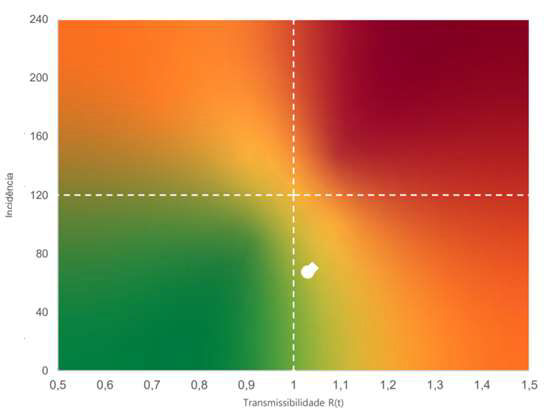
\includegraphics[width=0.95\columnwidth]{images/matrix.png}}
\caption{Matriz de risco}
\label{matrix}
\end{figure}
Para a criação do atributo ClassedeRisco, verificaram-se os valores de Rt e Incidência para atribuir as classes “Verde”, “Amarelo” e “Vermelho” com base na Matriz de Risco Fig.\ref{matrix}.
Após esta classificação, verificaram-se o número de países que estão em cada região, tendo obtido os seguintes valores:
Verde – 55
Amarelo – 34
Vermelho – 120
Mais uma vez, a maioria dos países encontra-se na zona com os piores valores (zona vermelha), tendo o valor do Rt um contributo significativo, como observado nas conclusões do ponto '\ref{ex05}'.



\subsection{Avaliação da capacidade preditiva relativamente ao novo atributo ClassedeRisco usando árvore de regressão, rede neuronal e k-vizinhos-mais-próximos.}
\subsubsection{Árvore de decisão}
A árvore de regressão foi criada de maneira idêntica aos exercícios anteriores com o método “class”, uma vez que este atributo exige uma análise classificativa dos dados. A árvore obtida encontra-se presente na Fig.\ref{8a_rpart}.
\begin{figure}[htbp]
\centerline{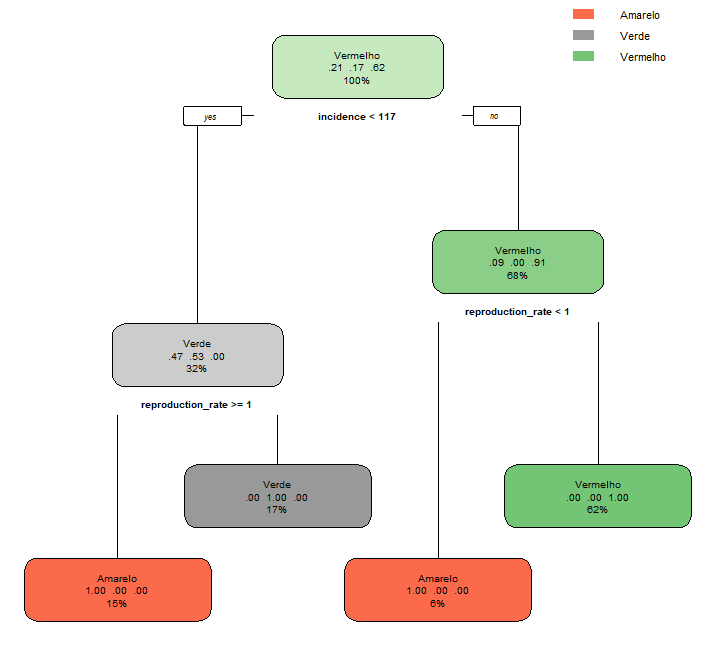
\includegraphics[width=0.95\columnwidth]{images/08_1.png}}
\caption{Árvore de decisão para a varíavel ClassedeRisco}
\label{8a_rpart}
\end{figure}
Com o modelo obtido, obtiveram-se os valores de avaliação presentes na Fig.\ref{8a_confusionmatrix}.
\begin{figure}[htbp]
\centerline{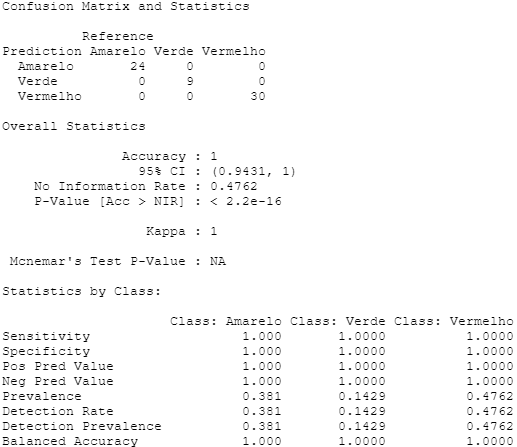
\includegraphics[width=0.95\columnwidth]{images/08_2.png}}
\caption{Matriz de confusão e valores de avaliação do modelo da árvore de regressão}
\label{8a_confusionmatrix}
\end{figure}


\subsubsection{Rede neuronal}
Na preparação dos dados para a criação de uma rede neuronal, foi necessário utilizar os dados normalizados no ponto '\ref{ex01}' e também a coluna ClassedeRisco, criada no ponto anterior. Como os dados desta nova coluna são classificados, houve a necessidade de criar colunas extras que continham os valores de “true”/”false” que diferenciavam as classes.
Após esta preparação, foi criada a rede neuronal com 3 nós internos, podendo esta ser observada na Fig.\ref{8b_neural}.
\begin{figure}[htbp]
\centerline{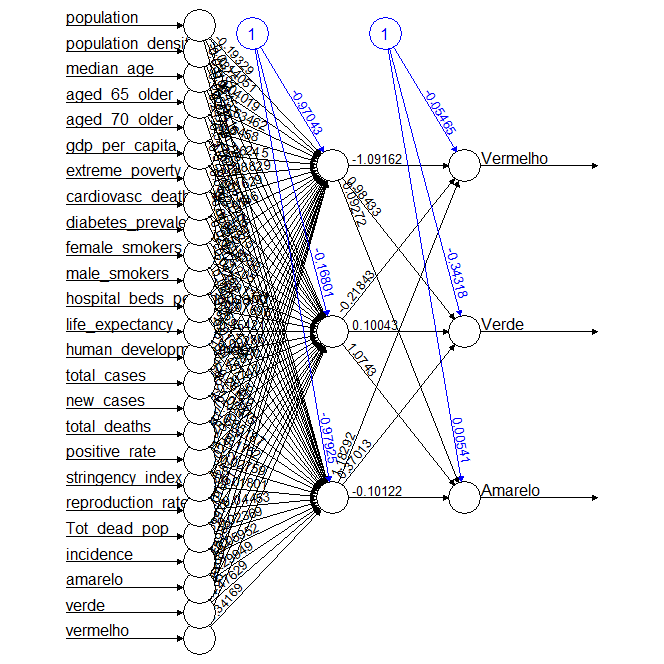
\includegraphics[width=0.95\columnwidth]{images/08_3.png}}
\caption{Rede neuronal com 3 nós internos para a varíavel ClassedeRisco}
\label{8b_neural}
\end{figure}
A Matriz de Confusão e os valores provenientes da mesma da rede neuronal criada estão indicados na Fig.\ref{8b_confusionmatrix}.
\begin{figure}[htbp]
\centerline{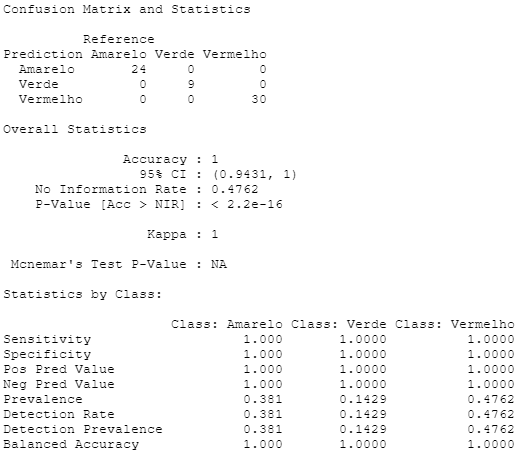
\includegraphics[width=0.95\columnwidth]{images/08_4.png}}
\caption{Matriz de confusão e valores de avaliação do modelo da rede neuronal}
\label{8b_confusionmatrix}
\end{figure}


\subsubsection{K-vizinhos-mais-próximos}
Antes da realização do algoritmo knn, foi necessária a separação da variável em estudo (“ClassedeRisco”) dos restantes dados de treino e teste. Após esta divisão, calculou-se o valor de k através da equação \eqref{6c_k}, com o resultado obtido presente na mesma.

\begin{figure}[htbp]
\centerline{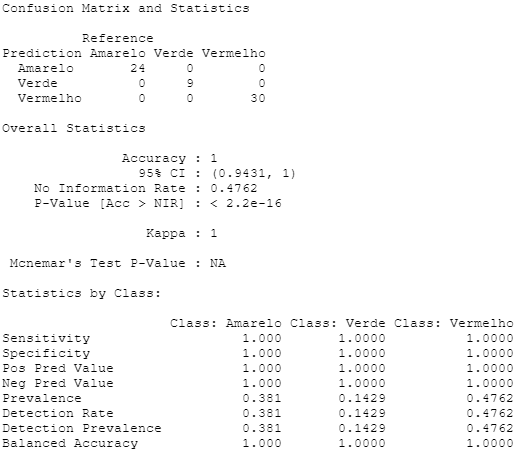
\includegraphics[width=0.95\columnwidth]{images/08_5.png}}
\caption{Matriz de confusão e valores de avaliação do modelo Knn}
\label{8c_confusionmatrix}
\end{figure}
Com os dados preparados e o valor de k encontrado, procedeu-se à realização do algoritmo e obtiveram-se os resultados dos valores de avaliação para este modelo, visíveis na Fig.\ref{8c_confusionmatrix}.

\subsubsection{Comparação dos modelos}
Com a realização destes três algoritmos e a posterior obtenção da matriz de confusão com os valores de \textit{Accuracy}, \textit{Precision} (na matriz de confusão referida como “Pos/Neg Pred Value”), \textit{Sensitivity} e \textit{Specificity}, sendo estes os máximos possíveis, conclui-se que todos os algoritmos tiverem um desempenho excelente, não tendo falhado nenhuma previsão durante o período de testagem. O valor de F1 resultante para todos os algoritmos é também de 1.
Assim, este problema de classificação acabou por ser algo bastante simples para todos os algoritmos utilizados conseguirem prever os dados sem quaisquer tipos de erros.



\section{Conclusões} % ------------------------------------------------------
As alíneas referentes a problemas de Regressão permitem concluir que o algoritmo de regressão linear simples não se revelou um modelo forte, não só pela sua fraca correlação como pela dispersão de pontos visível no diagrama obtido. Os métodos de avaliação MAE e RMSE confirmam a sua avaliação negativa. O mesmo se concluiu para a regressão linear múltipla, tendo sido o pior modelo face às redes neuronais e árvore de regressão. 

Já nos problemas de Classificação verificou-se, em primeiro lugar, que a maioria dos países tem índice de transmissibilidade superior a 1 e à média dos países em geral. Relativamente aos algoritmos, as redes neuronais e knn demonstraram ser os melhores face à árvore de decisão, sendo que o método de avaliação k-fold cross validation confirma que as redes neuronais foram ainda superiores ao knn. Contudo, na última alínea todos estes algoritmos obtiveram um resultado perfeito, não se verificando diferenças na avaliação dos mesmos. Por fim, denotou-se que a maioria dos países encontra-se na zona vermelha da matriz de risco, obtendo as classificações de: 55 países verdes, 34 amarelos e 120 vermelhos. 

Em suma, é visível que a regressão linear apresenta sempre piores resultados, quer a simples, quer a múltipla, face aos restantes algoritmos. As árvores de regressão ou decisão revelam-se melhores que os anteriores mas continuam inferiores face às redes neuronais ou knn, sendo estes os melhores algoritmos dos testes realizados. 



\begin{thebibliography}{00}

\bibitem{database} Ritchie, H. (2021, 31 de maio). \textit{Coronavirus Source Data}. Our World in Data. \url{https://ourworldindata.org/coronavirus-source-data}

\bibitem{dataFile} Our World in Data (2021, 31 de maio). [Ficheiro Csv]

\bibitem{algorithms} Brownlee, J. (2019, 12 de agosto). \textit{A Tour of Machine Learning Algorithms}. Machine Learning Mastery. \url{https://machinelearningmastery.com/a-tour-of-machine-learning-algorithms/}

\bibitem{regressionalgorithms} Ohri, J. (2017, 16 de fevereiro). \textit{Popular Regression Algorithms In Machine Learning Of 2021}. Jigsaw Academy. \url{https://www.jigsawacademy.com/popular-regression-algorithms-ml/}

\bibitem{clusteringalgorithms} McGregor, M, (2020, 21 de setembro). \textit{8 Clustering Algorithms in Machine Learning that All Data Scientists Should Know}. Free Code Camp. \url{https://www.freecodecamp.org/news/8-clustering-algorithms-in-machine-learning-that-all-data-scientists-should-know/ }

\bibitem{associationrulealgorithms} Shaier, S. (2019, 18 de março). \textit{ML Algorithms: One SD - Association Rule Learning Algorithms}. Towards Data Science. \url{https://medium.com/@Shaier/ml-algorithms-one-sd-\%CF\%83-association-rule-learning-algorithms-b35303e215d}

\bibitem{evaluationmetrics} Mansah. (2020, 24 de novembro). \textit{A Tour of Evaluation Metrics for Machine Learning}. Analytics Vidhya. \url{https://www.analyticsvidhya.com/blog/2020/11/a-tour-of-evaluation-metrics-for-machine-learning/}

\bibitem{knn} Lateef, Z. (2020, 14 de maio). \textit{KNN Algorithm: A Practical Implementation Of KNN Algorithm In R}. Edureka! \url{https://www.edureka.co/blog/knn-algorithm-in-r/}

\end{thebibliography}

\end{document}
